\documentclass[12pt]{article}
\usepackage{geometry}                % See geometry.pdf to learn the layout options. There are lots.
\geometry{letterpaper}                   % ... or a4paper or a5paper or ... 
%\geometry{landscape}                % Activate for for rotated page geometry
\usepackage[parfill]{parskip}    % Activate to begin paragraphs with an empty line rather than an indent
\usepackage{daves,fancyhdr,natbib,graphicx,dcolumn,amsmath,lastpage,url}
\usepackage{amsmath,amssymb,epstopdf,longtable}
\usepackage[final]{pdfpages}
\DeclareGraphicsRule{.tif}{png}{.png}{`convert #1 `dirname #1`/`basename #1 .tif`.png}
\pagestyle{fancy}
\lhead{CE 3354 -- Engineering Hydrology}
\rhead{FALL 2024}
\lfoot{ES4}
\cfoot{}
\rfoot{Page \thepage\ of \pageref{LastPage}}
\renewcommand\headrulewidth{0pt}



\begin{document}
\begin{center}
{\textbf{{ CE 3354 Engineering Hydrology} \\ {Exercise Set 4}}}
\end{center}

\section*{\small{Exercises}}
\begin{enumerate}
\item Use the Oklahoma data you prepared in ES-3 and analyze using the Bulletin 17C procedure (using the PeakFQ software tool - use station skew option).   \\~\\ If starting from just the data in ES3 you will have to carefully build an input file -- the \textbf{Beargrass-B17C.txt}\footnote{This file is located in same directory as this document} file is the correct format. 

\textbf{Solution}

The \textbf{Beargrass-B17C.txt} file is shown below

\begin{verbatim}
* WCF2.DATA  1/9/89 -- BULLETIN 17 EXAMPLES
*---+----1----+----2----+----3----+----4----+----5----+----6----+----7----+----8

Z                               USGS

*               LAT   LON                        AREA          ELEV
* STATIONID     DDMMSSDDDMMSS                    1234567123456712345678

H 12345678      3527470973329                    645.55        1202.01
N 12345678      OKLAHOMA FROM ES3
Y 12345678      20.0
2 12345678
3 12345678      19230101 200000
3 12345678      19240101 42000
3 12345678      19250101 11300
3 12345678      19260101 32400
3 12345678      19270101 108000
3 12345678      19280101 73000
3 12345678      19290101 76500
3 12345678      19300101 47800
3 12345678      19310101 28200
3 12345678      19320101 33700
3 12345678      19330101 25700
3 12345678      19340101 11700
3 12345678      19350101 77800
3 12345678      19360101 26600
3 12345678      19370101 47500
3 12345678      19380101 75600
3 12345678      19390101 19200
3 12345678      19400101 27800
3 12345678      19410101 51000
3 12345678      19420101 94000
3 12345678      19430101 97200
3 12345678      19440101 179000
3 12345678      19450101 124000
3 12345678      19460101 110000
3 12345678      19470101 114000
3 12345678      19480101 70200
3 12345678      19490101 70700
3 12345678      19500101 92800
3 12345678      19510101 135000
3 12345678      19520101 25800
3 12345678      19530101 17500
3 12345678      19540101 18700
3 12345678      19550101 36300
3 12345678      19560101 49200
3 12345678      19570101 120000
3 12345678      19580101 56800
3 12345678      19590101 54800
3 12345678      19600101 158000
3 12345678      19610101 165000
3 12345678      19620101 103000
3 12345678      19630101 19700
3 12345678      19640101 21100
3 12345678      19650101 171000
3 12345678      19660101 10400
3 12345678      19670101 42000
3 12345678      19680101 52800
3 12345678      19690101 77000
3 12345678      19700101 101000
3 12345678      19710101 17100         
*
\end{verbatim}

Now load this file into PeakFQ, adjust the settings (EMA, and set skew to \textsl{station skew}), like below

\begin{figure}[h!] %  figure placement: here, top, bottom, or page
   \centering
   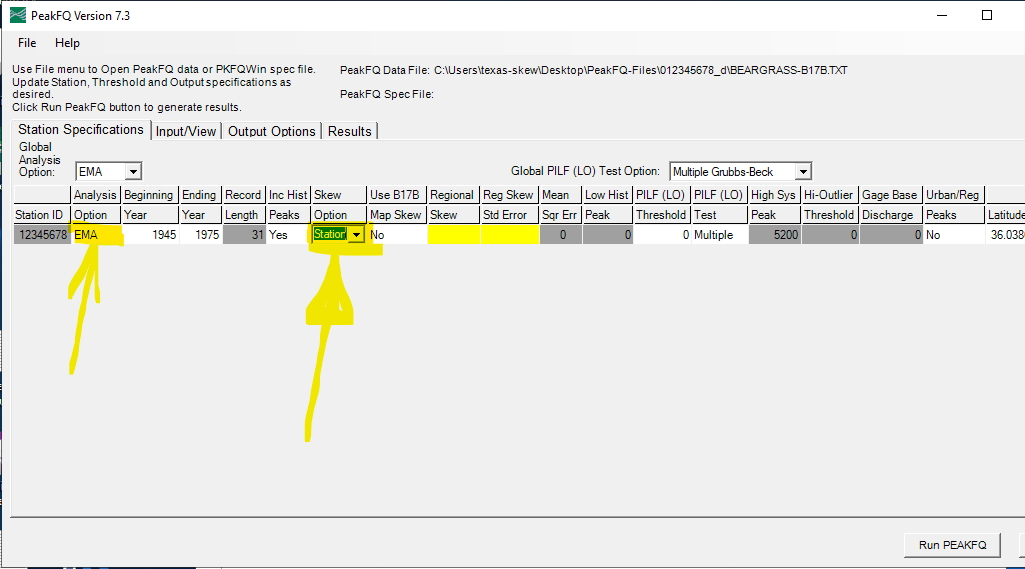
\includegraphics[width=6in]{BeargrassPFQSetuo.png} 
   \caption{PeakFQ 7.3 Set up screen for Beargrass Creek Data Analysis}
   \label{fig:BeargrassPFQSetuo}
\end{figure}

\clearpage

Then run the program and extract results (either graphically, or using the output file Table 4)

\begin{figure}[h!] %  figure placement: here, top, bottom, or page
   \centering
   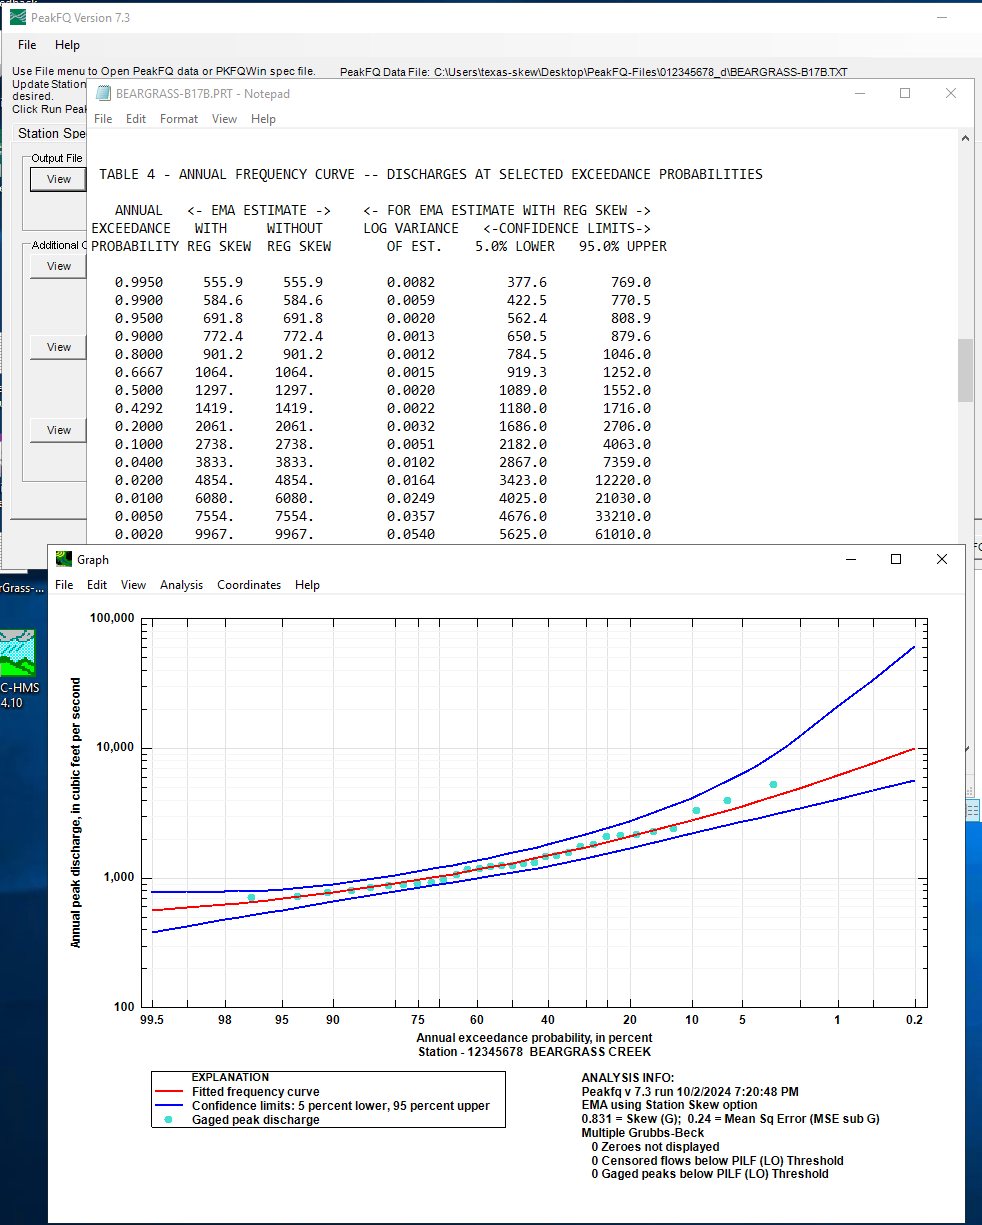
\includegraphics[height=6in]{BeargrassPFQRun.png} 
   \caption{PeakFQ 7.3 results for Beargrass Creek Data Analysis}
   \label{fig:BeargrassPFQRun}
\end{figure}
\clearpage

\item  Locate USGS Station 08144800 Brady Creek near Eden, TX. and analyze the historical peaks using the Bulletin 17C procedures (using the PeakFQ software tool use station skew option).  Determine the median discharge predicted for this station by PeakFQ.  Also determine the discharge per square mile of contributing drainage area.

\textbf{Solution}

\begin{figure}[h!] %  figure placement: here, top, bottom, or page
   \centering
   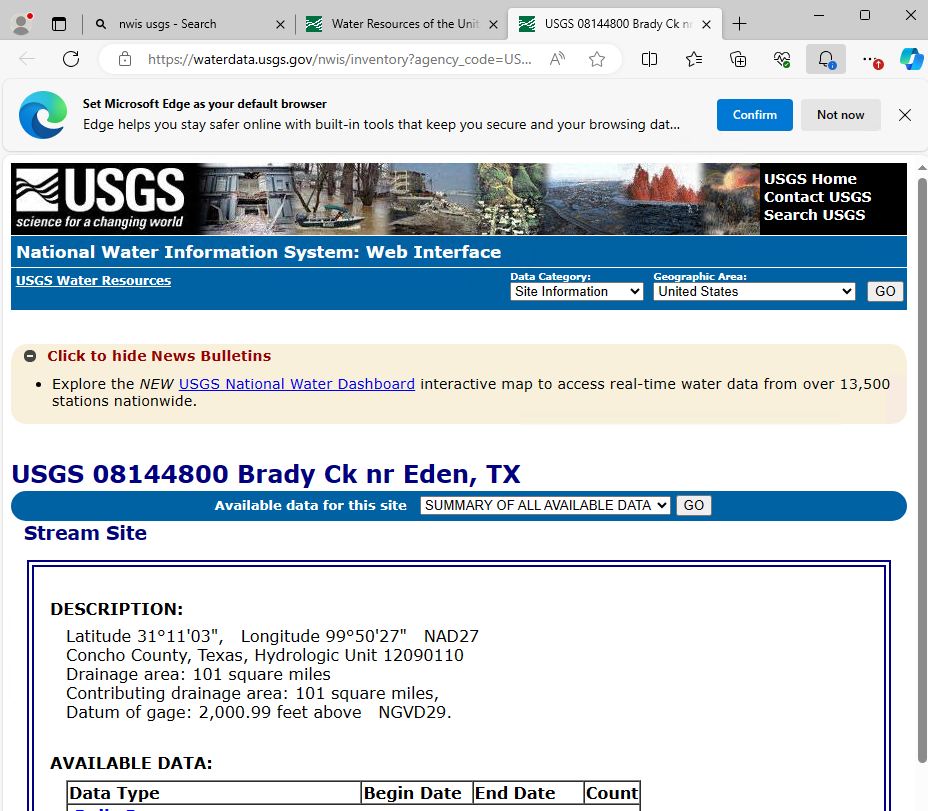
\includegraphics[width=6in]{BradyCreek.png} 
   \caption{Find NWIS data for Brady Creek Data Analysis}
   \label{fig:BradyCreek}
\end{figure}

\clearpage

The \textbf{Brady Creek STA\_08144800.txt} file is shown below

\begin{verbatim}
Z08144800                       USGS 
H08144800       3111030995027004848095SW12090110101    101     2000.99          
N08144800       Brady Ck nr Eden, TX
Y08144800       
308144800       19611009    2786               3.18                      
308144800       19630505   3.006               1.45                      
308144800       19631001   0.006                                         
308144800       19650518   57.06               2.24                      
308144800       19660428   51106               7.08                      
308144800       19670817   45606               6.72                      
308144800       19680310   11.06               1.78                      
308144800       19690911    9466               4.37                      
308144800       19700515   12.06               1.83                      
308144800       19710530   10206               4.04                      
308144800       19720615    3756               3.00                      
308144800       19730603    4106               3.07                      
308144800       19731012   33206               6.16                      
308144800       19750511    2446               3.07                      
308144800       19760711    4736               3.51                      
308144800       19770624   37206               6.45                      
308144800       19780528   38.06               1.84                      
308144800       19790809   10.06               1.51                      
308144800       19800909   13506               4.58                      
308144800       19810516   48.06               2.03                      
308144800       19820505    1776               2.71                      
308144800       19830606    1356               2.55                      
308144800       19840812    3336               3.14                      
308144800       19841231   60.06               2.08  
\end{verbatim}

\begin{figure}[h!] %  figure placement: here, top, bottom, or page
   \centering
   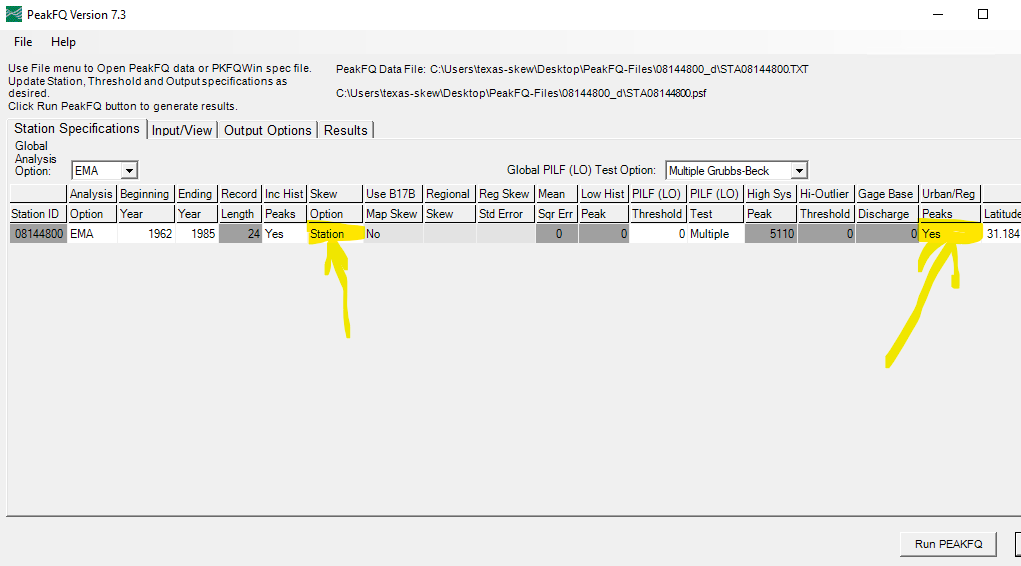
\includegraphics[width=6in]{BradyCreekSetup.png} 
   \caption{PeakFQ 7.3 setup for Brady Creek Data Analysis}
   \label{fig:BradyCreekSetuo}
\end{figure}

Then run the program and extract results (either graphically, or using the output file Table 4)

\begin{figure}[h!] %  figure placement: here, top, bottom, or page
   \centering
   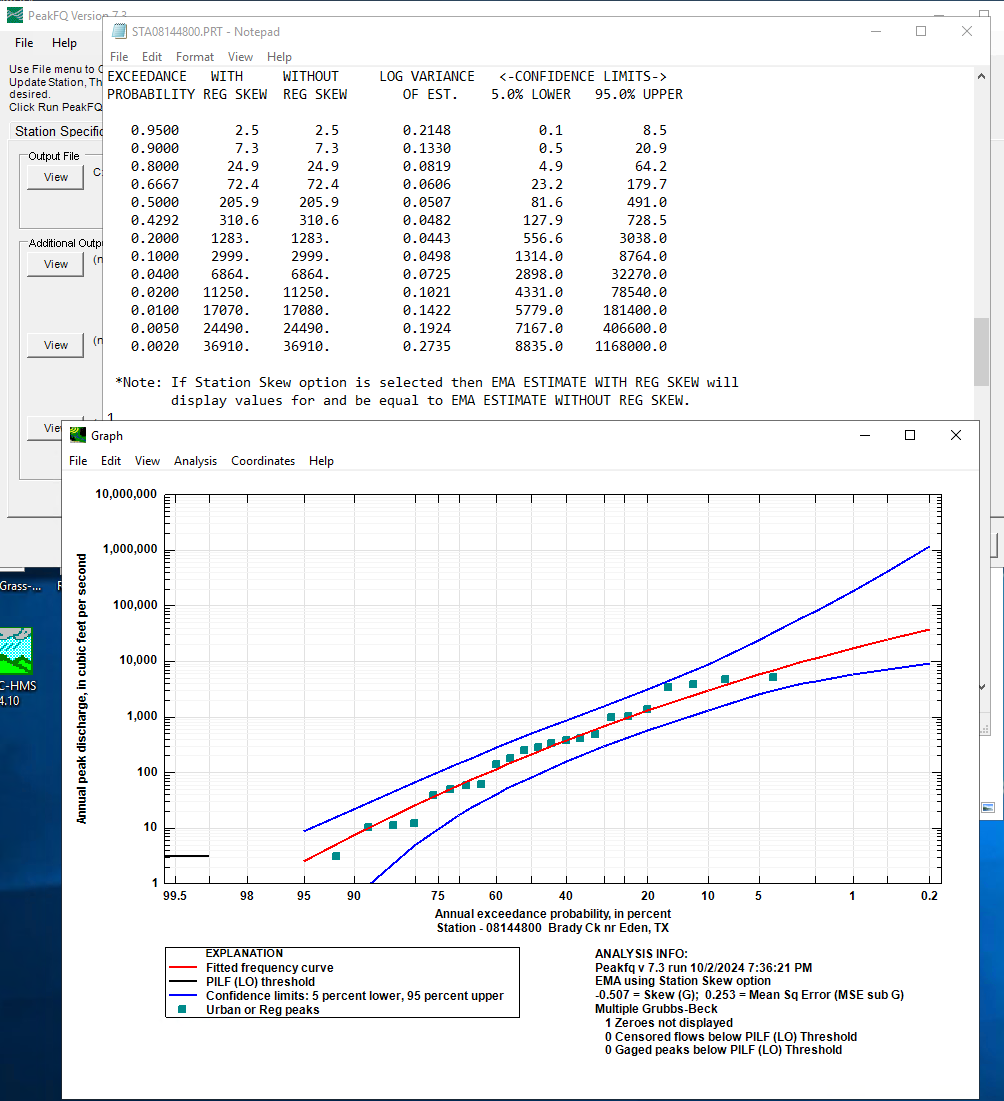
\includegraphics[width=6in]{BradyCreekPFQRun.png} 
   \caption{PeakFQ 7.3 results for Brady Creek Data Analysis}
   \label{fig:BradyCreekPFQRun}
\end{figure}

\clearpage

Median discharge is 205.9 CFS (Table 4 50\% exceedance probability)
Median Discharge per square mile is $\frac{205.9~cfs}{101~mi^2} = 2.04~\frac{cfs}{mi^2}$, can also apply to other probabilities.  This value is useful to check that the smallish drainage area for the study is producing resonable estimates.

\item  Use the NOAA Precipitation Frequency Data Server to prepare Intensity-Duration-Frequency curves for Eden, Texas (Concho County).   The desired ARI are 2-yr, 10-yr, 50-yr, and 100-yr (4 curves).\\

\textbf{Solution}

\begin{figure}[h!] %  figure placement: here, top, bottom, or page
   \centering
   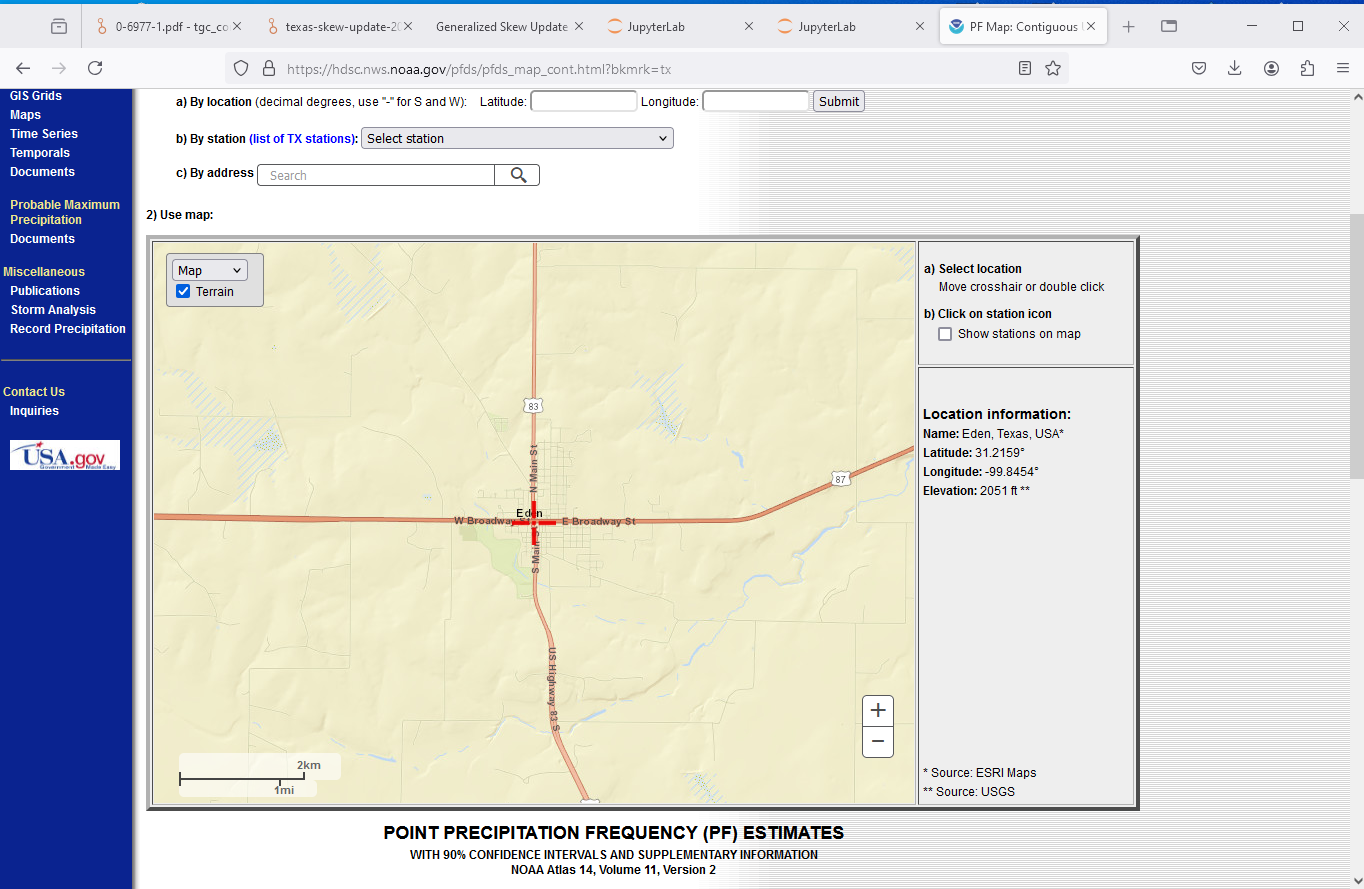
\includegraphics[width=6in]{EdenPFDSLocate.png} 
   \caption{NOAA PFDS landing page for Eden, Tx.}
   \label{fig:EdenPFDSLocate}
\end{figure}

\begin{figure}[h!] %  figure placement: here, top, bottom, or page
   \centering
   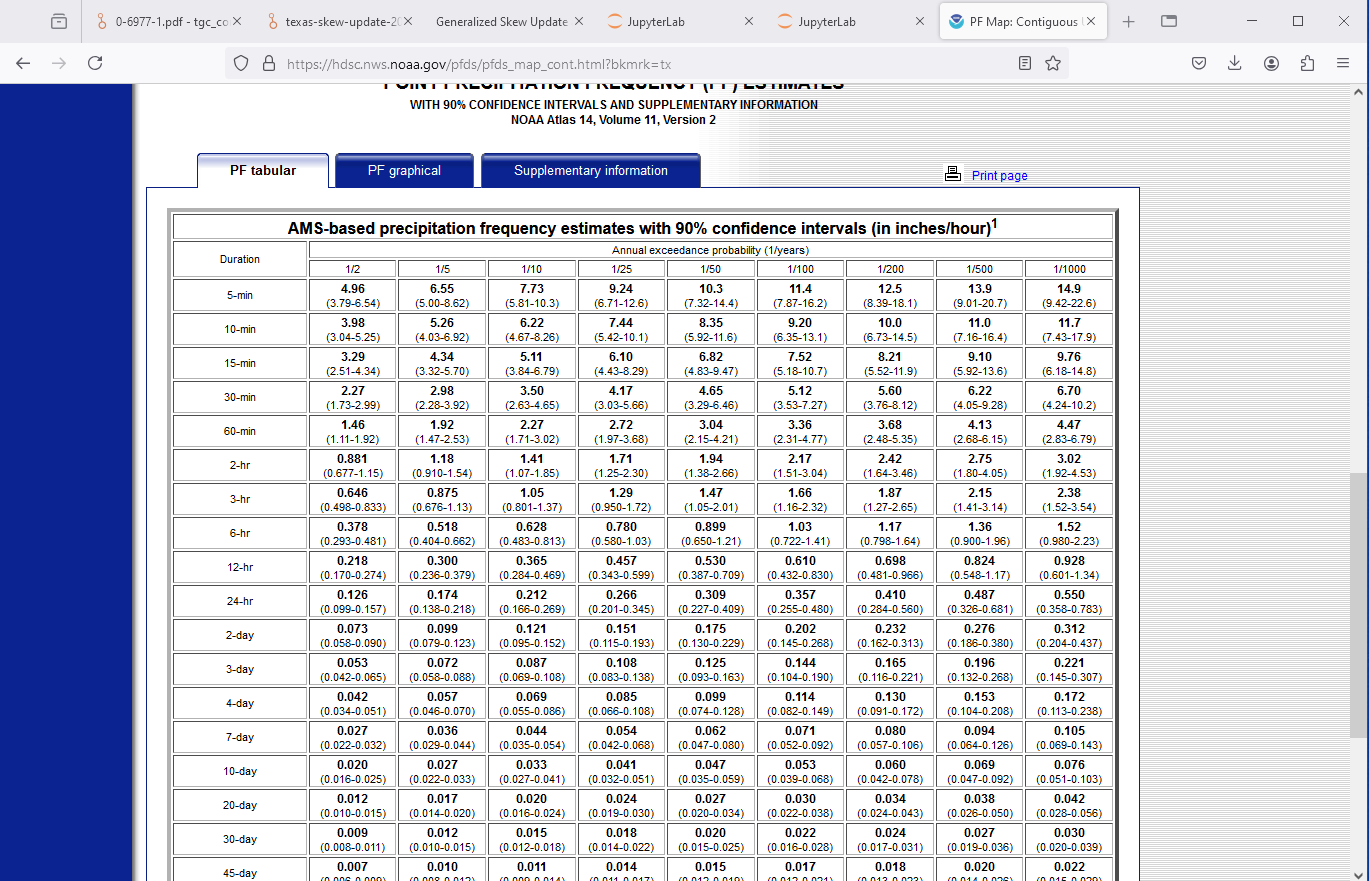
\includegraphics[width=6in]{EdenPFDSTabular.png} 
   \caption{NOAA PFDS Tabular Results for Eden, Tx.}
   \label{fig:EdenPFDSTabular}
\end{figure}

\begin{figure}[h!] %  figure placement: here, top, bottom, or page
   \centering
   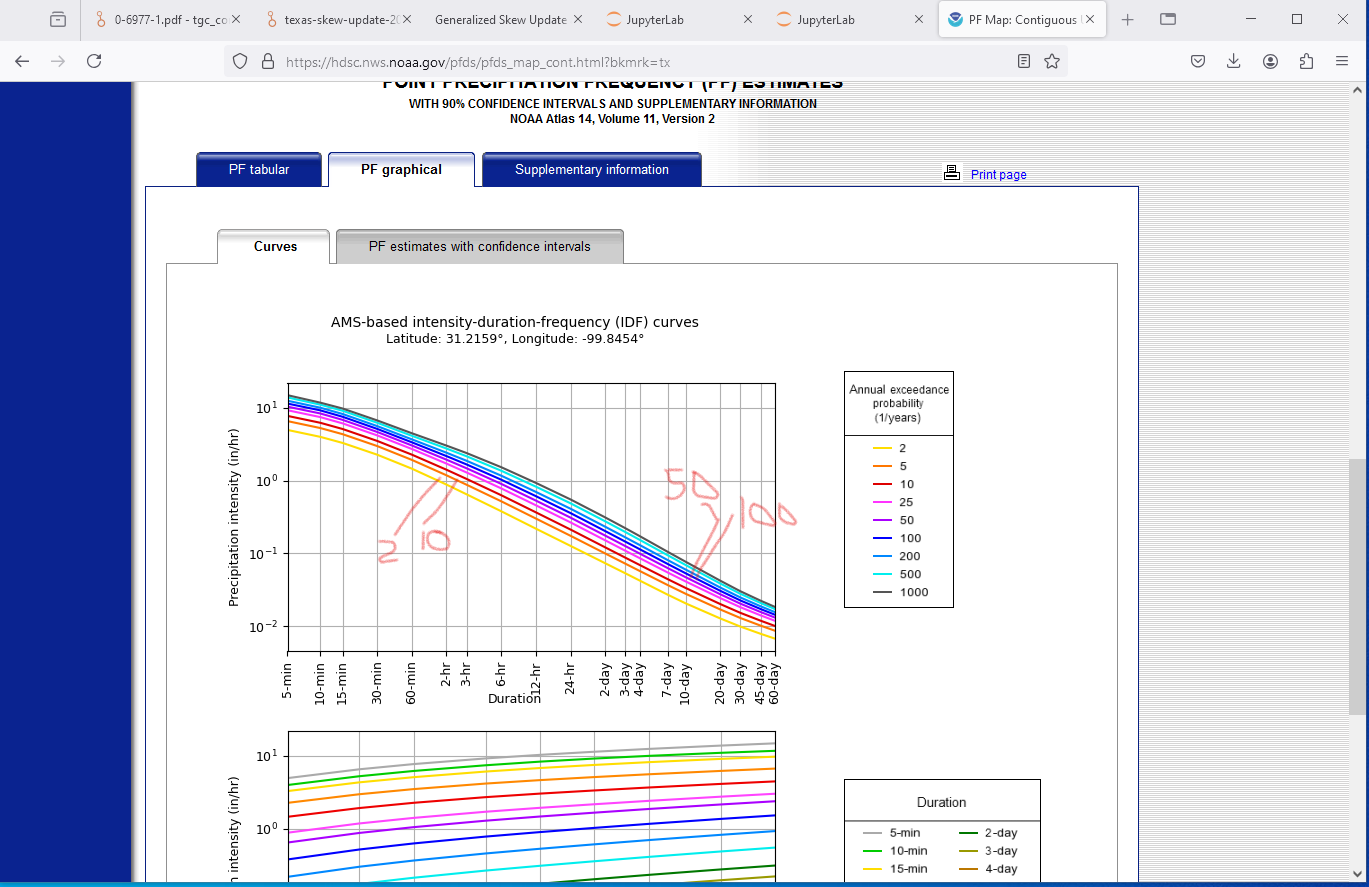
\includegraphics[width=6in]{EdenPFDSCurves.png} 
   \caption{NOAA PFDS Charts for Eden, Tx.}
   \label{fig:EdenPFDSCurves}
\end{figure}

In practice, use the tabular part to build own charts, as the online charts are not useable (except to check your homebrew work)

\clearpage

\item Use the NOAA Precipitation Frequency Data Server and the SCS Rainfall Distributions to prepare a 50-yr, 24-hour hyetograph for Eden, Texas.\\

\textbf{Solution}

Find the 50-yr, 24-hr depth from PFDS, which is 7.44 inches.  Then construct SDS distribution using ENGR-1330 methods

\begin{figure}[h!] %  figure placement: here, top, bottom, or page
   \centering
   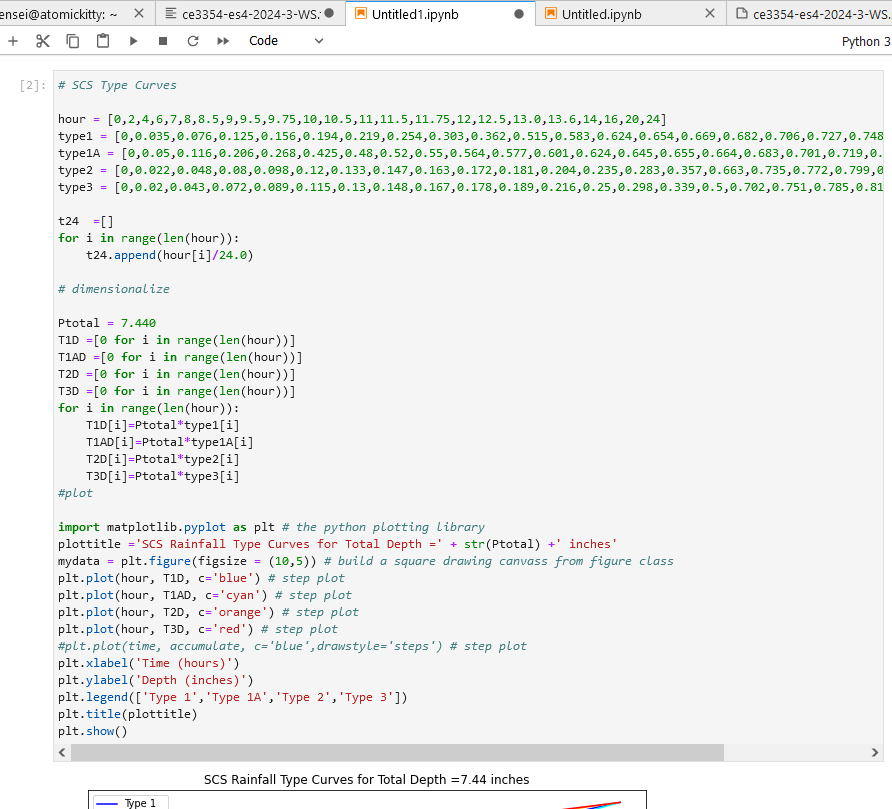
\includegraphics[width=6in]{EdenSCS1.png} 
   \caption{SCS generation script from class notes}
   \label{fig:EdenSCS1}
\end{figure}

\begin{figure}[h!] %  figure placement: here, top, bottom, or page
   \centering
   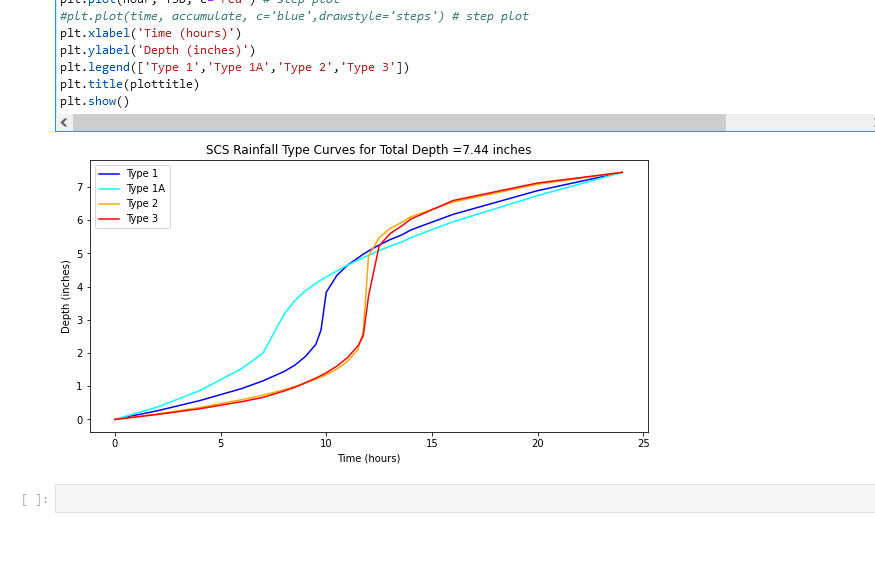
\includegraphics[width=6in]{EdenSCS2.png} 
   \caption{SCS Hyetographs}
   \label{fig:EdenSCS2}
\end{figure}

\clearpage

\item Use the NOAA Precipitation Frequency Data Server and the Texas Hyetograph Tool (TxHYETO-2015.xlsx) to prepare a 50-yr, 24-hour hyetograph for Eden, Texas.\\

\textbf{Solution}

Using the same total depth employ the \texttt{TXHYETO-2015.xls} tool:

\begin{figure}[h!] %  figure placement: here, top, bottom, or page
   \centering
   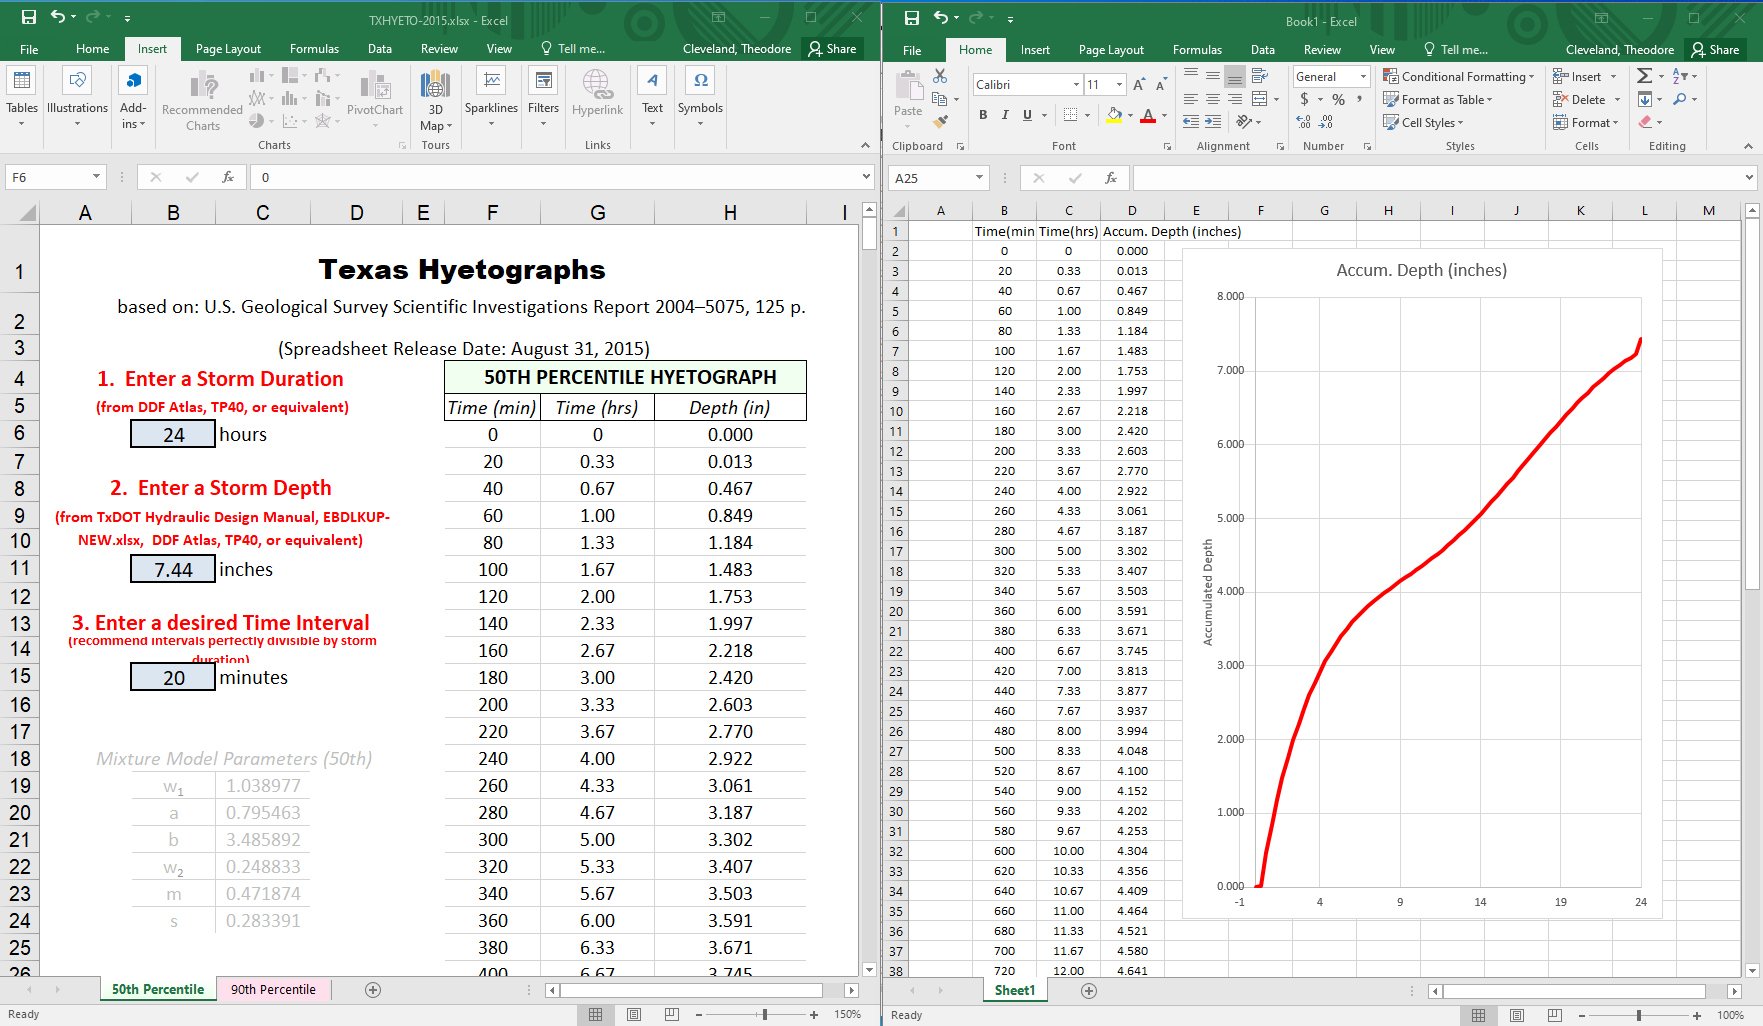
\includegraphics[width=6in]{EdenTxhyeto.png} 
   \caption{Texas 50\% Hyetograph}
   \label{fig:EdenTxhyeto}
\end{figure}

\end{enumerate}

\textbf{Save these 50-yr, 24-hour hyetograph for Eden, Texas.; you will reuse them as inputs for the Hardin Branch project.}

\clearpage

\section*{\small{Beargrass-B17C in PeakFQ format (minor editing may still be needed)}}
\begin{verbatim}
* WCF2.DATA  1/9/89 -- BULLETIN 17 EXAMPLES
*---+----1----+----2----+----3----+----4----+----5----+----6----+----7----+----8

Z                               USGS

*               LAT   LON                        AREA          ELEV
* STATIONID     DDMMSSDDDMMSS                    1234567123456712345678

H 12345678      3527470973329                    645.55        1202.01
N 12345678      OKLAHOMA FROM ES3
Y 12345678      20.0
2 12345678
3 12345678      19230101 200000
3 12345678      19240101 42000
3 12345678      19250101 11300
3 12345678      19260101 32400
3 12345678      19270101 108000
3 12345678      19280101 73000
3 12345678      19290101 76500
3 12345678      19300101 47800
3 12345678      19310101 28200
3 12345678      19320101 33700
3 12345678      19330101 25700
3 12345678      19340101 11700
3 12345678      19350101 77800
3 12345678      19360101 26600
3 12345678      19370101 47500
3 12345678      19380101 75600
3 12345678      19390101 19200
3 12345678      19400101 27800
3 12345678      19410101 51000
3 12345678      19420101 94000
3 12345678      19430101 97200
3 12345678      19440101 179000
3 12345678      19450101 124000
3 12345678      19460101 110000
3 12345678      19470101 114000
3 12345678      19480101 70200
3 12345678      19490101 70700
3 12345678      19500101 92800
3 12345678      19510101 135000
3 12345678      19520101 25800
3 12345678      19530101 17500
3 12345678      19540101 18700
3 12345678      19550101 36300
3 12345678      19560101 49200
3 12345678      19570101 120000
3 12345678      19580101 56800
3 12345678      19590101 54800
3 12345678      19600101 158000
3 12345678      19610101 165000
3 12345678      19620101 103000
3 12345678      19630101 19700
3 12345678      19640101 21100
3 12345678      19650101 171000
3 12345678      19660101 10400
3 12345678      19670101 42000
3 12345678      19680101 52800
3 12345678      19690101 77000
3 12345678      19700101 101000
3 12345678      19710101 17100         
*

\end{verbatim}

\clearpage
\section*{\small{Station 08144800 in PeakFQ format (minor editing may still be needed)}}
\begin{verbatim}
Z08144800                       USGS 
H08144800       3111030995027004848095SW12090110101    101     2000.99          
N08144800       Brady Ck nr Eden, TX
Y08144800       
308144800       19611009    2786               3.18                      
308144800       19630505   3.006               1.45                      
308144800       19631001   0.006                                         
308144800       19650518   57.06               2.24                      
308144800       19660428   51106               7.08                      
308144800       19670817   45606               6.72                      
308144800       19680310   11.06               1.78                      
308144800       19690911    9466               4.37                      
308144800       19700515   12.06               1.83                      
308144800       19710530   10206               4.04                      
308144800       19720615    3756               3.00                      
308144800       19730603    4106               3.07                      
308144800       19731012   33206               6.16                      
308144800       19750511    2446               3.07                      
308144800       19760711    4736               3.51                      
308144800       19770624   37206               6.45                      
308144800       19780528   38.06               1.84                      
308144800       19790809   10.06               1.51                      
308144800       19800909   13506               4.58                      
308144800       19810516   48.06               2.03                      
308144800       19820505    1776               2.71                      
308144800       19830606    1356               2.55                      
308144800       19840812    3336               3.14                      
308144800       19841231   60.06               2.08  
\end{verbatim}

\end{document}  